\chapter{デザイン指針}
\label{chapter:design_guidline}
本章では,提案システムのデザイン指針について述べる.

\section{対象とする状況}
\label{section:target_situation}
  本研究では,\ref{section:purpose}節で述べた目的を実現するために,都市部や繁華街などの店舗が多数存在している地域において,観光客などその地域に慣れていないユーザが携帯端末を手に持ち,
  (1)看板などの周囲の視覚情報が多すぎるため,目的地の看板は目に入っているものの,周辺の過剰な視覚情報に埋没して,素早く見つけることが困難である状況,
  (2)目の前にある店舗の情報が知りたいが,その地域に慣れていないことや言語障壁などの問題によって,その店舗の詳細情報を知ることが困難である状況,
  の2つの状況を対象とする.

  (1)に対しては,過剰に存在する視覚情報の中から,ユーザにとって不要な情報を低減することによって,情報の視認性の向上を実現する.この手法を``減算型表示''と定義し,視覚情報が密集している地域においてユーザが必要とする情報を素早く発見できるシステムを実装する.
  (2)に対しては,看板画像を認識し,オープンデータを用いてから店舗情報を取得することによって,目の前にある店舗の詳細情報を直感的かつ容易に得られるようにする.この手法を``Search by Snap''と定義し,ユーザが店舗の看板にモバイルデバイスのカメラを向けるだけでその店舗の情報が得られるシステムを実装する.
  
\section{提案システムの要件}
  \label{subsection:requirement}
  \ref{section:target_situation}節で述べた問題を解決し,素早く目的の情報にアクセスするために必要な要件として,以下の4点を定義する.
  \begin{enumerate}
    \item ユーザが求める店舗情報の探索が直感的にできる操作方法であること
    \item ユーザがカメラを通して見た店舗の看板と端末の画面上に表示される付加情報とのシームレスな連携が可能であること
    \item 周囲に店舗が密集している場合においても,ユーザが必要とする看板情報を迷わずに探索できること
    \item 天候や時間帯などの環境条件に左右されず,ユーザに迷わせることなく情報の提示ができること
  \end{enumerate}
  本稿で提案するシステムは,モバイルデバイス上で実行することを想定している.システムを実現するにあたり,上述した(1)と(2)を満たすために,
  \begin{itemize}
    \item ユーザが店舗名や店舗の種類をクエリとして検索するために,システムを利用する地域における店舗の種類,名称及びその看板画像の組がデータベースとして用意されていること
    \item リアルタイムで看板認識を行うために,モバイルデバイスは動画の撮影が可能であり,端末上またはサーバ上でリアルタイムで画像処理が行える環境が存在すること
    \item サーバ上にあるデータベースにアクセスするために,Long Term Evolution(LTE)やWi-Fiなどの方法でインターネットにアクセスできること
    \item 歩きながら端末を操作することは危険であり,ユーザは立ち止まって片方の手でモバイルデバイスを持ち,もう片方の手でシステム操作を行うことが望ましいため,片手で操作できるサイズの端末であること
  \end{itemize}
  の4点を前提条件として想定する.

\section{減算型表示}
\label{section:dr_method}
  これまでの研究動向として,藤田らは,ARを用いて情報を重畳することで必要な情報を目立たせる手法を「加算型の情報提示」,DRのアプローチを取り入れることで不要な情報を目立たなくさせる手法を「減算型の情報提示」と位置付け,減算型情報提示手法を提案した\cite{Fujita:2013}.減算型情報提示手法において適切な情報削除の方法を検証するために,藤田らは以下に示す3種類の手法を用いて画像から不要な情報を減算し,情報探索の所要時間を計測する実験を行った.
  \begin{itemize}
    \item 白黒:不要な情報の彩度をなくしたもの
    \item ぼかし:不要な情報の輪郭情報をなくしたもの
    \item 白黒とぼかし:不要な情報の彩度と輪郭情報をなくしたもの
  \end{itemize}
  実験は,ユーザが街の中で減算型情報提示手法を用いたシステムを使うことを想定し,上記の手法で情報を減算した画像を携帯端末に表示して行われた.実験開始前に探索する看板の店舗名のみを実験参加者に教示し,その看板を見つけるよう指示を出した.実験開始から教示した看板を発見するまでの時間を計測した.実験の結果,探索時間は削減方法の差による影響を受けないことが示唆された.また,アンケートで最も良かった減算手法について質問したところ,白黒が過半数を超えた.そこで本研究では,情報の削減手法に白黒を用いて実験を行う.藤田らの実験では実験は看板の多い環境において減算型情報提示手法の優位性を確認するために,既存の情報にARを用いて情報を加算する従来の手法(加算型情報提示手法)と,DRのアプローチを用いて不要な情報を減算する提案手法(減算型情報提示手法)との比較を行い,それぞれの探索時間を比較が行われた.加算型情報提示手法を適用する画像は,画像の中にある探索対象の看板に緑色の吹き出しを追加し,その中に店舗名を表示した.一方,減算型情報提示手法を適用する画像には,探索対象の看板以外の情報を白黒にした.実験から得られた探索時間の結果を比較したところ,減算型情報提示手法に優位性は見られなかった.このため,加算型情報提示手法と減算型情報提示手法には差がないことが示唆された.

  減算型情報提示手法の問題点として,不要な情報を減算する際,対象となる看板の色が白黒であり,かつその周辺の景色の彩度が低い場合がある.
  例として,新日本新地ビル\footnote{大阪府大阪市北区曾根先新地1-7-8}付近で撮影した図\ref{figure:kitashinchi}(a)の写真から,``春雨''以外の看板情報を減算すると,図\ref{figure:kitashinchi}(b)のようになる.
  このような場合,看板の視覚情報が減算された周囲の視覚情報と混同し,減算の効果が減少するという問題が生じる.
  この問題を解決するために,先行研究\cite{Kitamura:2017a, Kitamura:2017b}では,藤田らが提案した減算型情報提示手法を加算型で拡張し,加算型と減算型のハイブリッド型情報提示手法を提案した.

  \begin{figure}[t]
    \begin{minipage}{0.49\hsize}
        \begin{center}
            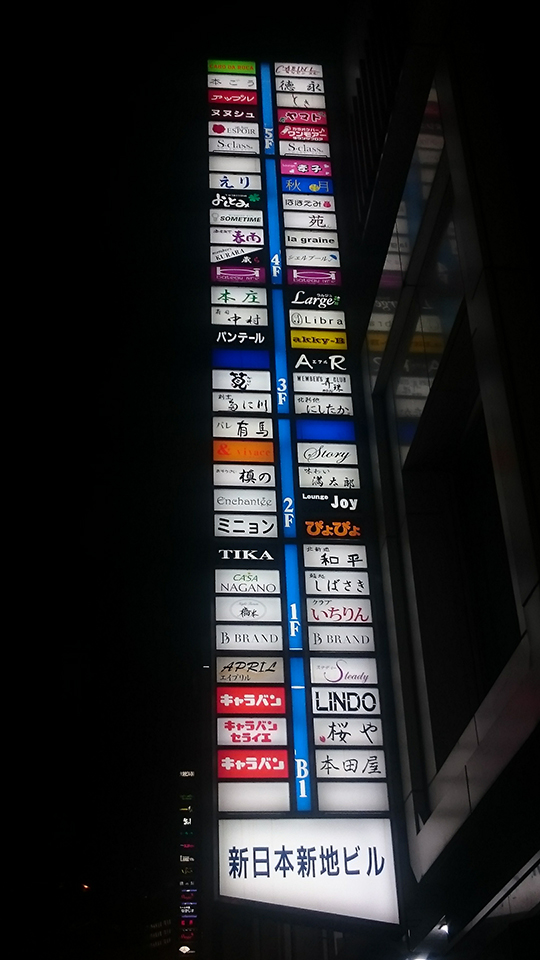
\includegraphics[clip, width=\textwidth]{kitashinchi1.png}\\
            \small{(a)加工前}
        \end{center}
    \end{minipage}
    \begin{minipage}{0.49\hsize}
        \begin{center}
            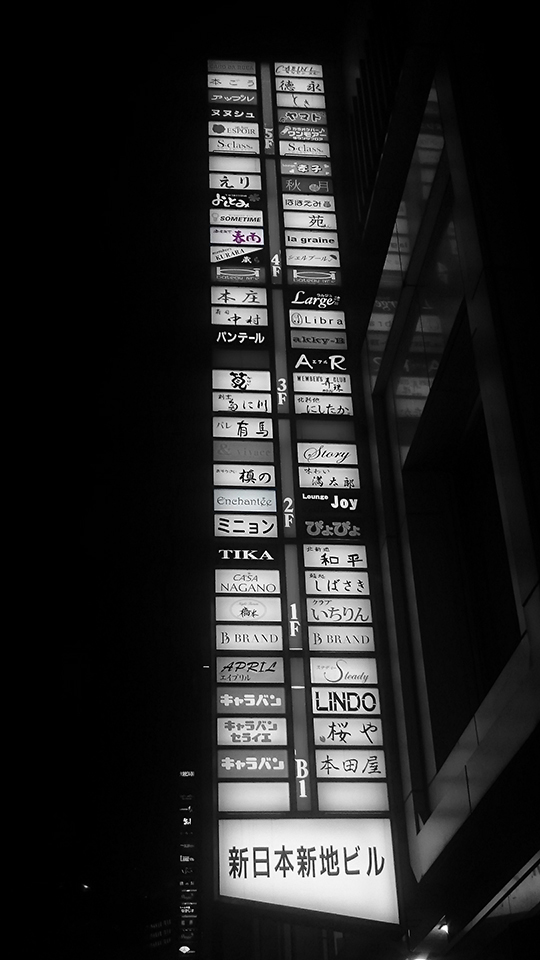
\includegraphics[clip, width=\textwidth]{kitashinchi2.png}\\
            \small{(b)加工後}
        \end{center}
    \end{minipage}
    \vspace{2pt}
    \caption{彩度が低い看板(文献\cite{Kitamura:2017a}より図引用)}
    \label{figure:kitashinchi}
  \end{figure}


  \subsection{提案インタフェースのデザイン}
    \ref{subsection:requirement}節の(3)を満たすために,文献\cite{Fujita:2013}で提案された減算型情報提示手法を用いる.しかし,不要な情報を減算するのみでは,周辺の景色の彩度が低い場合など,環境条件によっては減算の効果が得られないことがある.そこで\ref{subsection:requirement}節の(4)を満たすために,ARを用いて文字情報を付加したハイブリッド型情報提示手法を提案する.文字色は背景の色に合わせて変化させる.これにより,ユーザが求める情報のみが分かりやすく提示されるため,上記の問題の解決が期待される.提案システムでは,ユーザが目的の店舗名や店舗の種類をクエリとして入力する.ユーザが入力したクエリに一致する視覚情報はユーザにとって必要な情報であり,それ以外の視覚情報は不要な情報である.そのため,情報の識別性向上を目的として,図\ref{figure:dr_method}に示すような出力をユーザに提示する.これは,不要な視覚情報をグレースケール化することによって減算し,必要な視覚情報には店舗名などの文字情報を看板の横に重畳して表示したものである.これにより,ユーザは不要な視覚情報を完全に失うことなく,必要な視覚情報のみを得られることが期待される.

    \begin{figure}[tb]
      \centerline{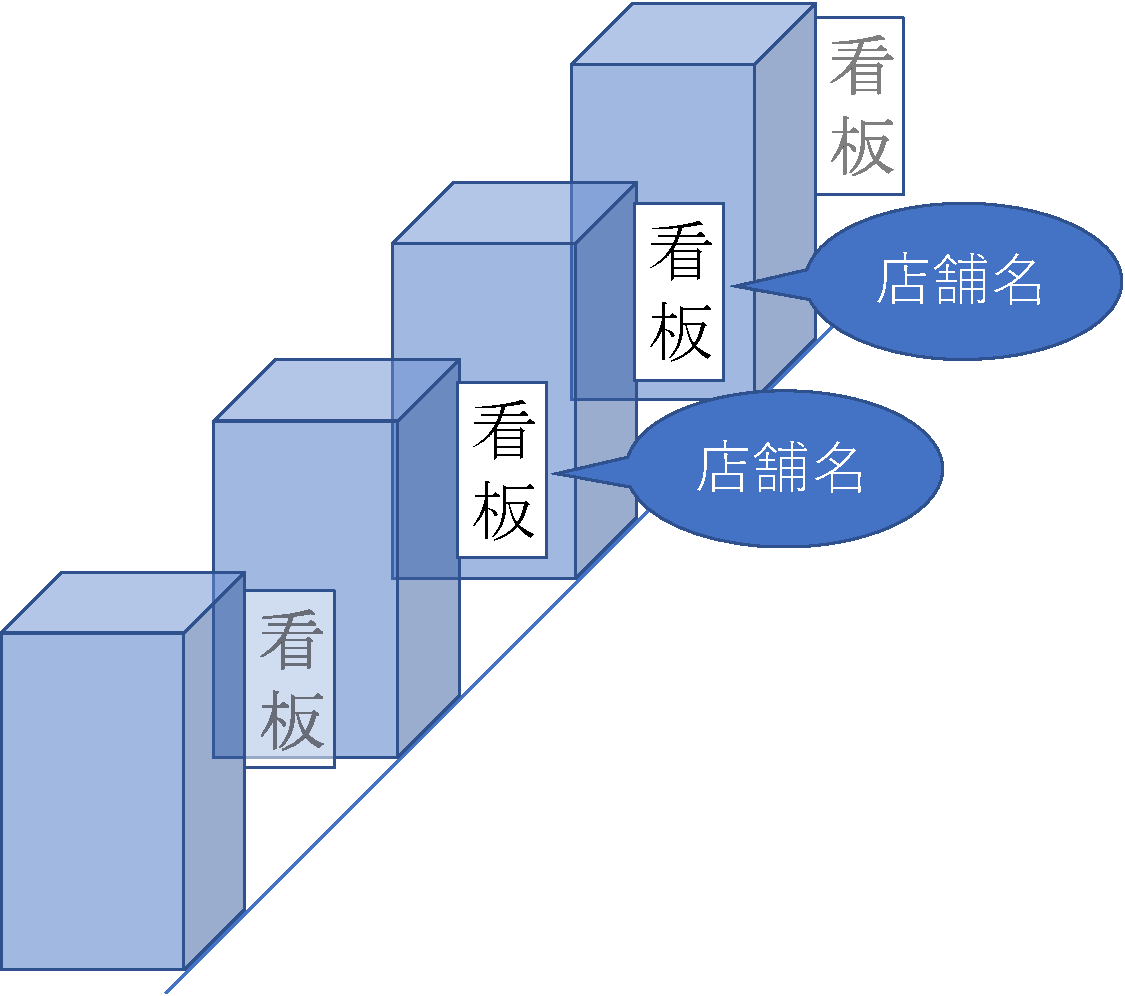
\includegraphics[width=\columnwidth, clip]{dr_method.pdf}}
      \caption{減算型表示の出力イメージ(文献\cite{Kitamura:2017a}より図引用)}
      \label{figure:dr_method}
    \end{figure}

\section{Search by Snap}
\label{section:design_sbs}
  \ref{section:searching_action}節で述べたように,ユーザが慣れていない地域や言語障壁のある地域において,目の前にある店舗で受けられるサービスの詳細やクレジットカードでの支払いの可否,店内での喫煙の可否,等の詳細情報を瞬時に把握することは困難である.
  この問題を解決するために,ユーザが携帯端末に搭載されているカメラを通して目の前の店舗の看板を見ることで,求める情報に素早くアクセスできるようにする.
  
  \subsection{提案インタフェースのデザイン}
    \ref{subsection:requirement}節で述べた(3)を満たすために,飲食店における予算や提供されている料理の種類,クレジットカードでの決済の可否など,ユーザが求めている条件をクエリとして入力でき,減算型表示のアプローチを用いてユーザにとって不要な情報は目立たなく表示するインタフェースとする.
    \ref{subsection:requirement}節の(4)を満たすために,減算型表示と同様に,条件に合致しない看板情報の色調を低減させ,条件に合う看板のみを強調して表示するインタフェースとする.
    提案インタフェースの出力イメージを図\ref{figure:sbs_method}に示す.
  \begin{figure}[tb]
    \centerline{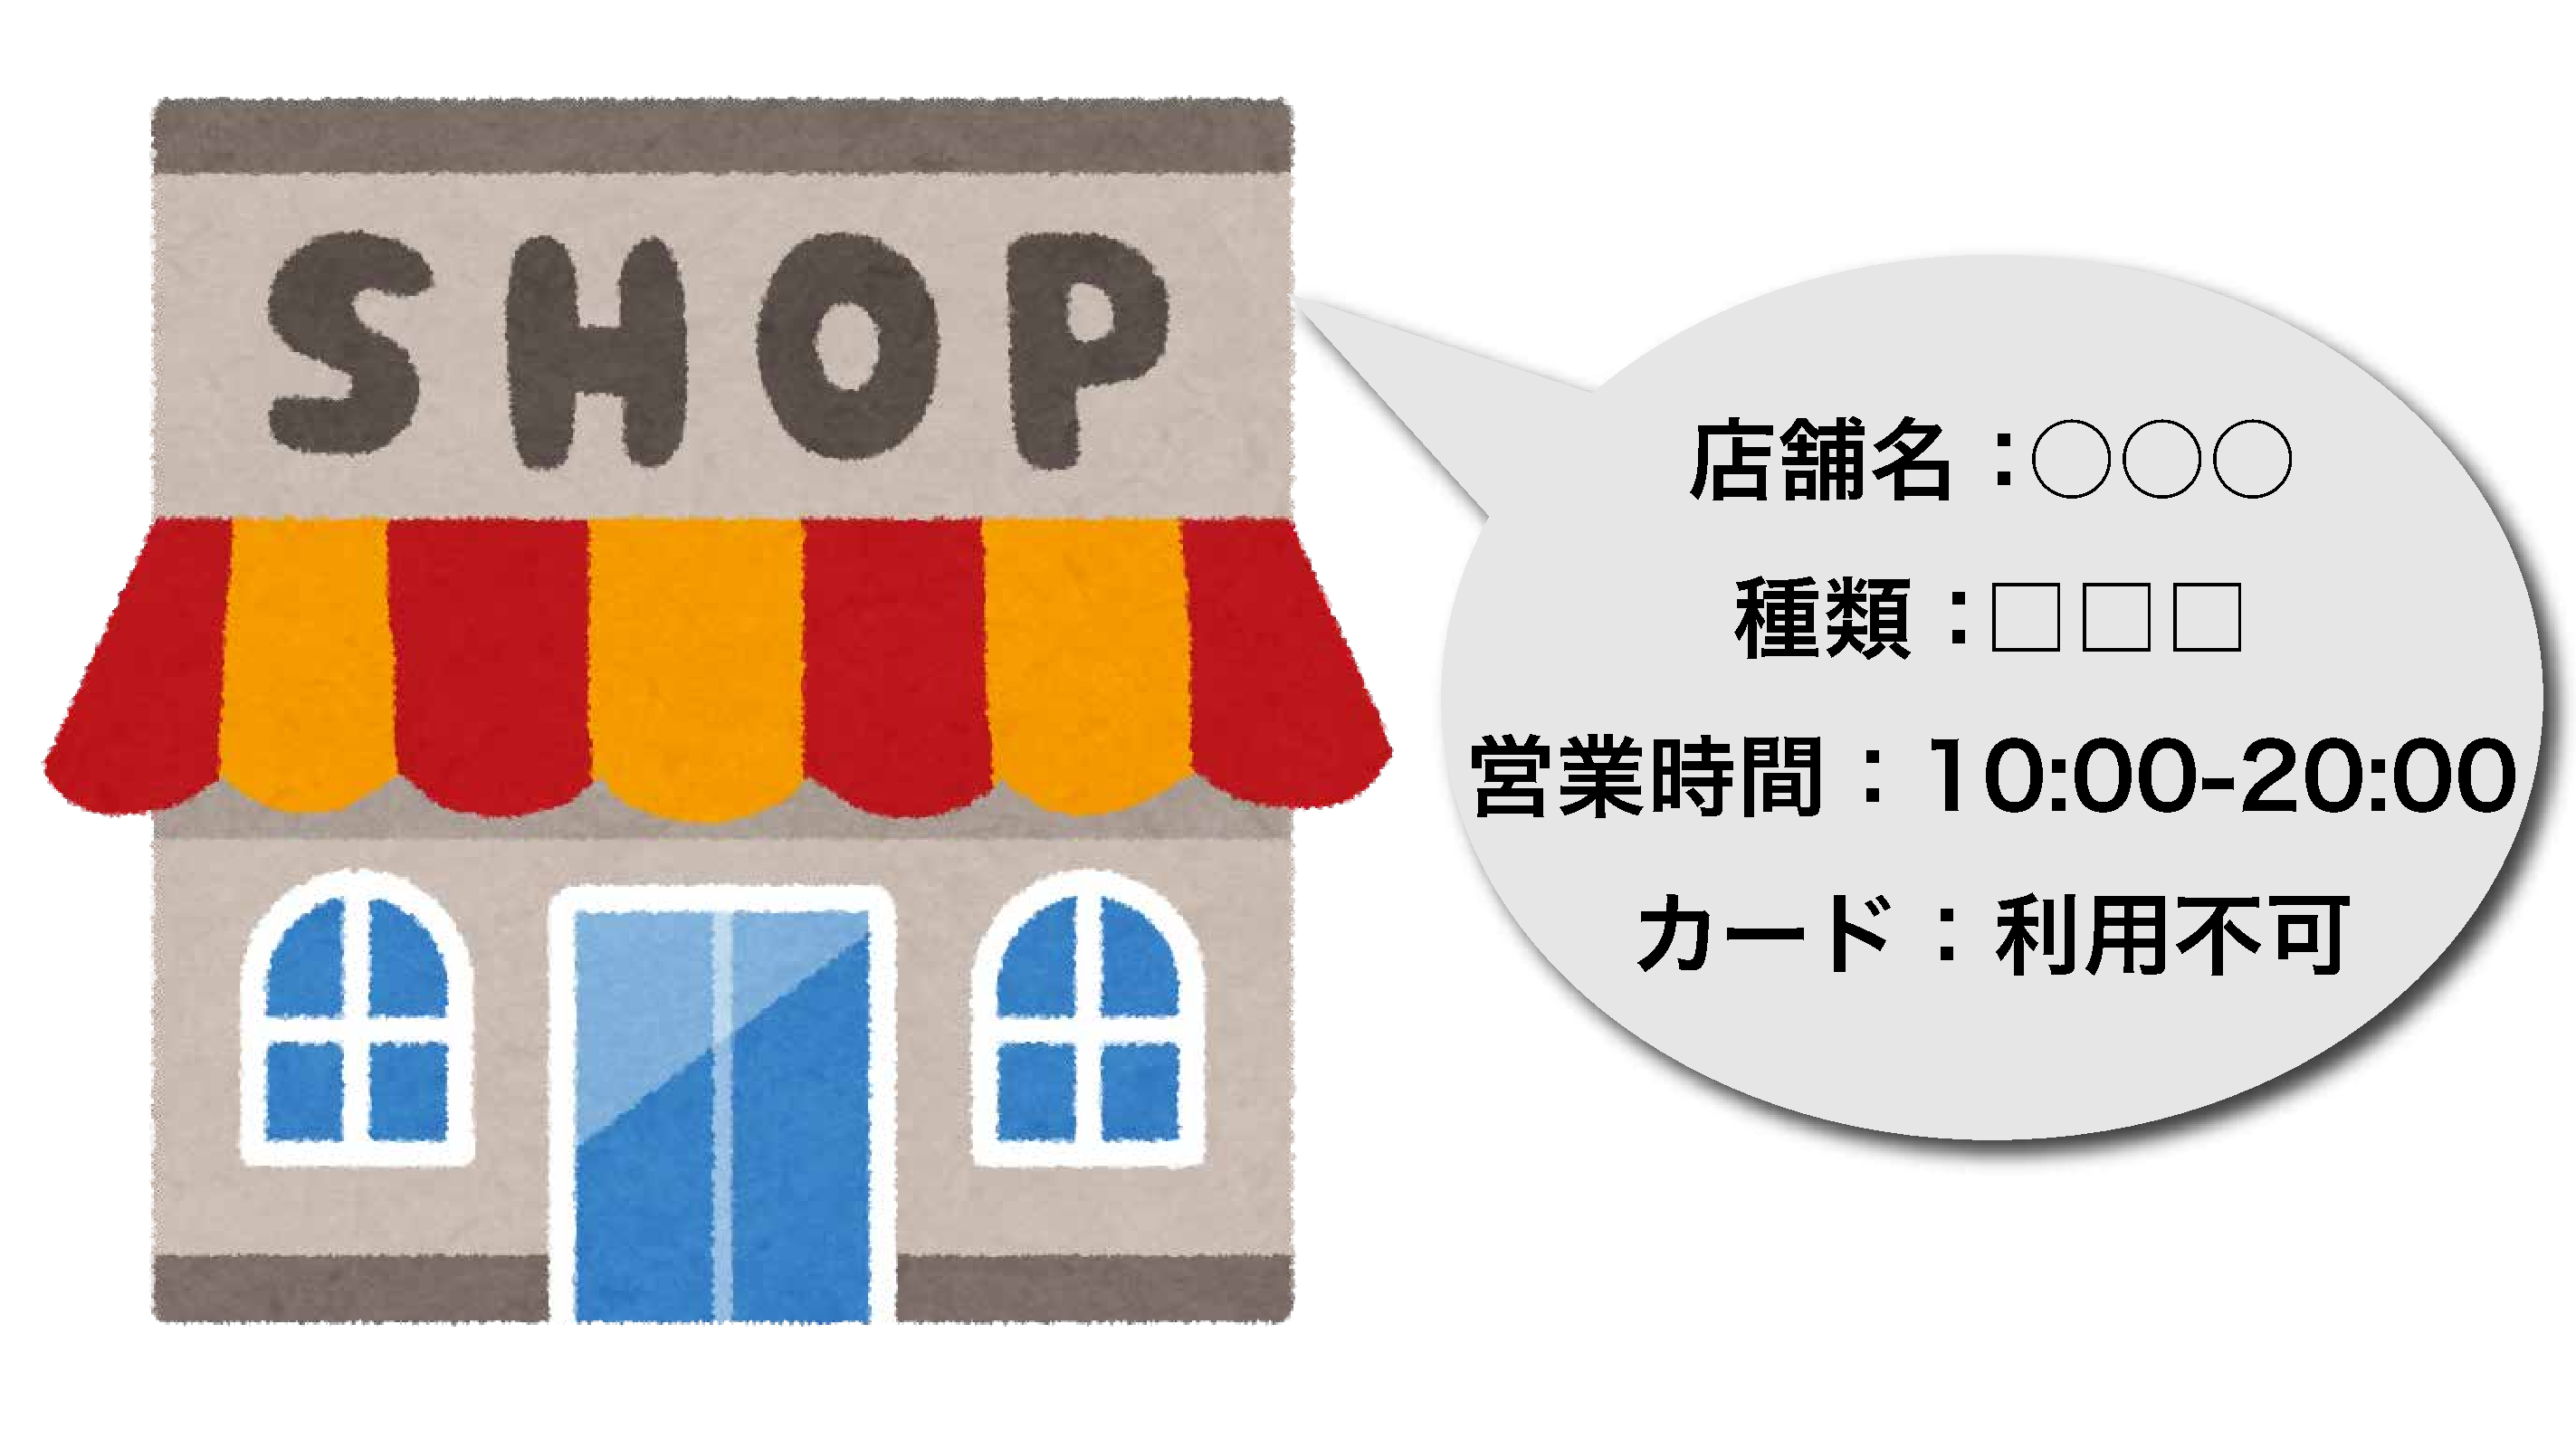
\includegraphics[width=\columnwidth, clip]{sbs_method.pdf}}
    \caption{Search by Snapの出力イメージ}
    \label{figure:sbs_method}
  \end{figure}